\subsection{Etude du lien entre âge et habitudes alimentaires}

\subsubsection{Préparation des données}

Nous avons ensuite voulu etudier le lien entre l'âge et les habitudes alimentaires.
Cepandant, la valeur du champ âge est directement l'âge, ce qui représente trop de catégories (une vingtaine) par rapport au nombre d'individus présent dans le jeu de données ($500$).
Nous avons donc décidé de répartir les individus en tranches d'âges: les $18-22$, $22-26$, $26-30$ et $30+$.
Nous pouvons maintenant voir dans le tableau de contingence en figure \ref{tab:contTableAgeDietary} que le nombre d'individus est suffisament élevé dans chaque catégorie pour pouvoir faire une AFC ayant du sens.

\begin{figure}[!h]
\begin{center}
  \begin{tabular}{|c|c|c|c|}
    \hline 
    & \multicolumn{3}{|c|}{Dietary Habits}\\ 
    \hline
    Age & Healthy & Moderate & Unhealthy \\ 
    \hline 
    18-22 & 35 & 39 & 42 \\ 
    \hline 
    22-26 & 36 & 34 & 43 \\ 
    \hline 
    26-30 & 41 & 34 & 48 \\ 
    \hline 
    30+ & 49 & 65 & 36 \\ 
    \hline
  \end{tabular}
\end{center}
\caption{Table de contingence entre les habitudes alimentaires et les tranches d'âges}
\label{tab:contTableAgeDietary}
\end{figure}

\subsubsection{Test Chi-deux}

Après exécution du test Chi-deux, la p-valeur obtenue est de environ $6\%$ ce qui est au-dessus de la p-valeur usuellement utilisée pour ce test, mais n'en est pas non plus très éloignée.
Ainsi, nous avons tout de même décidé de poursuivre l'analyse car cette p-valeur semble indiquer au moins une faible corrélation entre les deux variables.

\subsubsection{Valeurs propres et cercle des corrélations}

Après exécution de l'AFC, les deux composantes principales obtenues expliquent $100\%$ de la variance, avec la première en expliquant environ $97\%$.
Ainsi, la quasi-totalité des corrélations seront montrées par la première composante, soit l'axe des abscisses du cercle des corrélations donné en figure \ref{fig:corrAgeDietary}.

\begin{figure}[!h]
  \begin{center}
    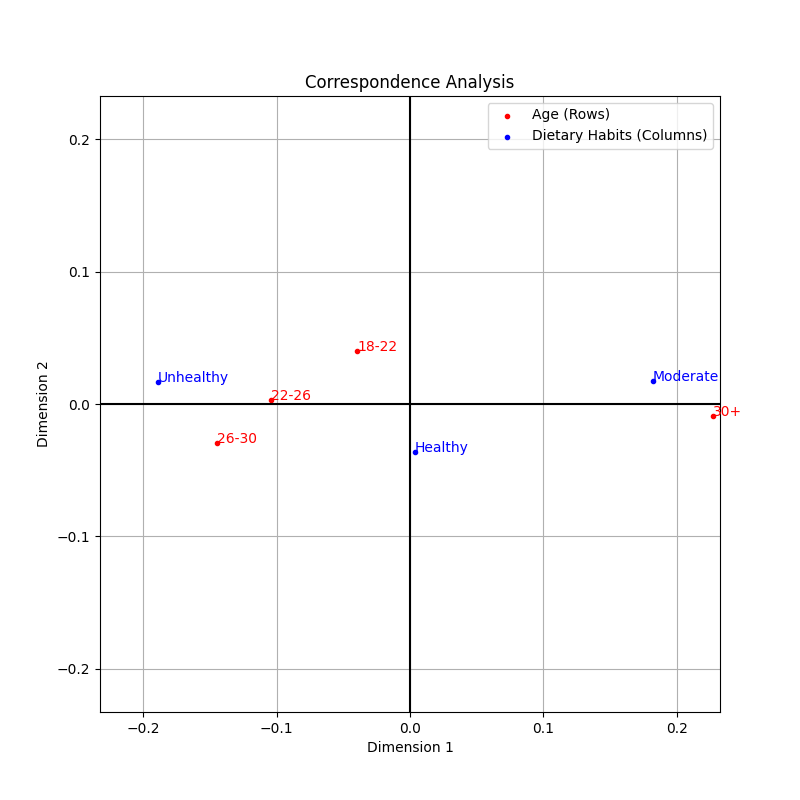
\includegraphics[width=0.55\textwidth]{Images/Age_Dietary_all/Corr_circle.png}
  \end{center}
  \caption{Cercle des corrélations de l'AFC sur les tranches d'âge et les habitudes alimentaires}
  \label{fig:corrAgeDietary}
\end{figure}

Sur la figure \ref{fig:corrAgeDietary}, on peut constater 2 légères tendances\footnote{Nous insistons vraiment sur le fait que ces corrélations sont faibles et ne représentent qu'au plus de légères tendances}:
\begin{itemize}
  \item Les plus de 30 ans ont tendance à avoir une alimentation modérée 
  \item Les 26-30 ans et 22-26 ans tendent quant à eux vers une alimentation plutôt mauvaise pour la santé
\end{itemize}

\subsubsection{Etude sur les données seulement avec dépressifs et sans dépressifs}

Lorsque que nous réalisons le test chi-deux sur le jeu de données sans les individus dépressifs et avec seulement les individus dépressifs, la p-valeur obtenue est respectivement de environ $51\%$ et de environs $42\%$, ce qui indique que les variables tranches d'âge et habitudes alimentaires sont indépendantes. 
Ceci peut être surprenant, étant donné qu'en faisant l'analyse avec la totalité des données, on obtient une faible corrélation. Il semblerait ici que la cause soit un effet similaire au paradoxe de Simpson \citep{simpson}, où une troisième variable est affectée par notre choix de séparation de la population, causant cette décorrélation. Cependant cela reste à confirmer.
